\documentclass[12pt, titlepage]{article}

\usepackage{fullpage}
\usepackage[round]{natbib}
\usepackage{multirow}
\usepackage{booktabs}
\usepackage{tabularx}
\usepackage{graphicx}
\usepackage{float}
\usepackage{hyperref}
\hypersetup{
    colorlinks,
    citecolor=blue,
    filecolor=black,
    linkcolor=red,
    urlcolor=blue
}


\newcounter{acnum}
\newcommand{\actheacnum}{AC\theacnum}
\newcommand{\acref}[1]{AC\ref{#1}}

\newcounter{ucnum}
\newcommand{\uctheucnum}{UC\theucnum}
\newcommand{\uref}[1]{UC\ref{#1}}

\newcounter{mnum}
\newcommand{\mthemnum}{M\themnum}
\newcommand{\mref}[1]{M\ref{#1}}

\begin{document}

\title{Module Guide for SCEC (Solar Cooker Energy Calculator)}
 
\author{Deesha Patel}
\date{\today}

\maketitle

\pagenumbering{roman}

\section{Revision History}

\begin{tabularx}{\textwidth}{p{3cm}p{2cm}X}
\toprule {\bf Date} & {\bf Version} & {\bf Notes}\\
\midrule
March 11, 2023 & 0.1 & Initial release\\
March 19, 2023 & 0.2 & Updates according to the comments \\ 
March 19, 2023 & 0.3 & Updates according to the issues \\ 
\bottomrule
\end{tabularx}

\newpage

\section{Reference Material}

This section records information for easy reference.

\subsection{Abbreviations and Acronyms}

\renewcommand{\arraystretch}{1.2}
\begin{tabular}{l l} 
  \toprule		
  \textbf{symbol} & \textbf{description}\\
  \midrule 
  AC & Anticipated Change\\
  DAG & Directed Acyclic Graph \\
  M & Module \\
  MG & Module Guide \\
  ODE & Ordinary Differential Equation \\ 
  OS & Operating System \\
  R & Requirement\\
  SC & Scientific Computing \\
  SCEC & Solar Cooker Energy Calculator\\
  SRS & Software Requirements Specification\\
  UC & Unlikely Change \\
  \bottomrule
\end{tabular}\\

\newpage

\tableofcontents

\listoftables

\listoffigures

\newpage

\pagenumbering{arabic}

\section{Introduction}

Decomposing a system into modules is a commonly accepted approach to developing
software.  A module is a work assignment for a programmer or programming
team~\citep{ParnasEtAl1984}.  We advocate a decomposition
based on the principle of information hiding~\citep{ParnasAndClements}.  This
principle supports design for change, because the ``secrets'' that each module
hides represent likely future changes.  Design for change is valuable in SC,
where modifications are frequent, especially during initial development as the
solution space is explored.  

Our design follows the rules layed out by \citet{ParnasEtAl1984}, as follows:
\begin{itemize}
\item System details that are likely to change independently should be the
  secrets of separate modules.
\item Each data structure is implemented in only one module.
\item Any other program that requires information stored in a module's data
  structures must obtain it by calling access programs belonging to that module.
\end{itemize}

After completing the first stage of the design, the Software Requirements
Specification (SRS), the Module Guide (MG) is developed~\citep{ParnasEtAl1984}. The MG
specifies the modular structure of the system and is intended to allow both
designers and maintainers to easily identify the parts of the software.  The
potential readers of this document are as follows:

\begin{itemize}
\item New project members: This document can be a guide for a new project member
  to easily understand the overall structure and quickly find the
  relevant modules they are searching for.
\item Maintainers: The hierarchical structure of the module guide improves the
  maintainers' understanding when they need to make changes to the system. It is
  important for a maintainer to update the relevant sections of the document
  after changes have been made.
\item Designers: Once the module guide has been written, it can be used to
  check for consistency, feasibility, and flexibility. Designers can verify the
  system in various ways, such as consistency among modules, feasibility of the
  decomposition, and flexibility of the design.
\end{itemize}

The rest of the document is organized as follows. Section
\ref{SecChange} lists the anticipated and unlikely changes of the software
requirements. Section \ref{SecMH} summarizes the module decomposition that
was constructed according to the likely changes. Section \ref{SecConnection}
specifies the connections between the software requirements and the
modules. Section \ref{SecMD} gives a detailed description of the
modules. Section \ref{SecTM} includes two traceability matrices. One checks
the completeness of the design against the requirements provided in the SRS. The
other shows the relation between anticipated changes and the modules. Section
\ref{SecUse} describes the use relation between modules.

\section{Anticipated and Unlikely Changes} \label{SecChange}

This section lists possible changes to the system. According to the likeliness
of the change, the possible changes are classified into two
categories. Anticipated changes are listed in Section \ref{SecAchange}, and
unlikely changes are listed in Section \ref{SecUchange}.

\subsection{Anticipated Changes} \label{SecAchange}

Anticipated changes are the source of the information that is to be hidden
inside the modules. Ideally, changing one of the anticipated changes will only
require changing the one module that hides the associated decision. The approach
adapted here is called design for
change.

\begin{description}
\item[\refstepcounter{acnum} \actheacnum \label{1_ac}:] The specific
  hardware on which the software is running.
\item[\refstepcounter{acnum} \actheacnum \label{2_ac}:] The format of the initial input data.
\item[\refstepcounter{acnum} \actheacnum \label{3_ac}:] The constraints on the input parameters. 
\item[\refstepcounter{acnum} \actheacnum \label{4_ac}:] How ODEs are defined using input parameters. 
\item[\refstepcounter{acnum} \actheacnum \label{5_ac}:] How the energy equations are calculated using input parameters. 
\item[\refstepcounter{acnum} \actheacnum \label{6_ac}:] The choice of data structure for sequence.
\item[\refstepcounter{acnum} \actheacnum \label{7_ac}:] The overall flow of the system. 
\item[\refstepcounter{acnum} \actheacnum \label{8_ac}:] The format of output data. 
\item[\refstepcounter{acnum} \actheacnum \label{9_ac}:] The algorithm to solve an ODE. 
\item[\refstepcounter{acnum} \actheacnum \label{10_ac}:] The implementation of plotting data. 


\end{description}

\subsection{Unlikely Changes} \label{SecUchange}

The module design should be as general as possible. However, a general system is
more complex. Sometimes this complexity is not necessary. Fixing some design
decisions at the system architecture stage can simplify the software design. If
these decision should later need to be changed, then many parts of the design
will potentially need to be modified. Hence, it is not intended that these
decisions will be changed.

\begin{description}
\item[\refstepcounter{ucnum} \uctheucnum \label{ucIO_1}:] Input/Output devices
  (Input: File and/or Keyboard, Output: File, Memory, and/or Screen).
\item[\refstepcounter{ucnum} \uctheucnum \label{ucInput_2}:] The source of input is always external to the software. 
\item[\refstepcounter{ucnum} \uctheucnum \label{ucOutput_3}:] The outputs are displayed on the output device. 
\item[\refstepcounter{ucnum} \uctheucnum \label{ucGoal_4}:] Goal of the system is to calculate the temperature and energy of the fluid.
\item[\refstepcounter{ucnum} \uctheucnum \label{ucEnergy_7}:] The implemented energy equation is reading inputs from the file.  

\end{description}

\section{Module Hierarchy} \label{SecMH}

This section provides an overview of the module design. Modules are summarized
in a hierarchy decomposed by secrets in Table \ref{TblMH}. The modules listed
below, which are leaves in the hierarchy tree, are the modules that will
actually be implemented.

\begin{description}
\item [\refstepcounter{mnum} \mthemnum \label{1_mHH}:] Hardware-Hiding Module
\item [\refstepcounter{mnum} \mthemnum \label{2_mHH}:] Constant Value Module
\item [\refstepcounter{mnum} \mthemnum \label{3_mHH}:] Energy Equation Module
\item [\refstepcounter{mnum} \mthemnum \label{4_mHH}:] Input Format Module
\item [\refstepcounter{mnum} \mthemnum \label{5_mHH}:] Input Parameter Module
\item [\refstepcounter{mnum} \mthemnum \label{6_mHH}:] Output Module
\item [\refstepcounter{mnum} \mthemnum \label{7_mHH}:] SCEC Control Module
\item [\refstepcounter{mnum} \mthemnum \label{8_mHH}:] Temperature ODE Module
\item [\refstepcounter{mnum} \mthemnum \label{9_mHH}:] ODE Solver Module
\item [\refstepcounter{mnum} \mthemnum \label{10_mHH}:] Plotting Result Module
\item [\refstepcounter{mnum} \mthemnum \label{12_mHH}:] Sequence Data Structure Module 

\end{description}


\begin{table}[h!]
\centering
\begin{tabular}{p{0.3\textwidth} p{0.6\textwidth}}
\toprule
\textbf{Level 1} & \textbf{Level 2}\\
\midrule
{Hardware-Hiding Module} & ~ \\
\midrule

\multirow{7}{0.3\textwidth}{Behaviour-Hiding Module} 
& Constant Value Module\\ 
& Energy Equation Module\\
& Input Format Module\\
& Input Parameter Module\\
& Output Module\\
& Control Module\\
& Temperature ODE Module\\
\midrule

\multirow{3}{0.3\textwidth}{Software Decision Module} 
& ODE Solver Module\\
& Plotting Result Module\\
& Sequence Data Structure Module\\
\bottomrule

\end{tabular}
\caption{Module Hierarchy}
\label{TblMH}
\end{table}

\section{Connection Between Requirements and Design} \label{SecConnection}

The design of the system is intended to satisfy the requirements developed in
the SRS. In this stage, the system is decomposed into modules. The connection
between requirements and modules is listed in Table~\ref{TblRT}.

\section{Module Decomposition} \label{SecMD}

Modules are decomposed according to the principle of ``information hiding''
proposed by \citet{ParnasEtAl1984}. The \emph{Secrets} field in a module
decomposition is a brief statement of the design decision hidden by the
module. The \emph{Services} field specifies \emph{what} the module will do
without documenting \emph{how} to do it. For each module, a suggestion for the
implementing software is given under the \emph{Implemented By} title. If the
entry is \emph{OS}, this means that the module is provided by the operating
system or by standard programming language libraries.  \emph{SCEC} means the
module will be implemented by the SCEC software.

Only the leaf modules in the hierarchy have to be implemented. If a dash
(\emph{--}) is shown, this means that the module is not a leaf and will not have
to be implemented.

\subsection{Hardware Hiding Modules (\mref{1_mHH})}

\begin{description}
\item[Secrets:]The data structure, algorithm and underlying hardware used to implement the virtual hardware.
\item[Services:]Serves as a virtual hardware used by the rest of the
  system. This module provides the interface between the hardware and the software. So, the SCEC system can use it to display outputs or to accept inputs.
\item[Implemented By:] OS
\end{description}

\subsection{Behaviour-Hiding Module}

\begin{description}
\item[Secrets:]The contents of the required behaviours.
\item[Services:]Includes programs that provide externally visible behaviour of
  the system as specified in the software requirements specification (\href{https://github.com/DeeshaPatel/CAS-741-Solar-Cooker/blob/2a6c0175891c01960d83cb99b73a762a9b2d2508/docs/SRS/SRS.pdf}{SRS})
  documents. This module serves as a communication layer between the
  hardware-hiding module and the software decision module. The programs in this
  module will need to change if there are changes in the SRS.
\item[Implemented By:] --
\end{description}

\subsubsection{Constant Value Module (\mref{2_mHH})}

\begin{description}
\item[Secrets:] The constant values used in the system. 
\item[Services:] Stores all the constant values in this module and responsible to provide them accordingly when needed to perform the operations in other modules. 
\item[Implemented By:] SCEC
\item[Type of Module:] Abstract Object 
\end{description}

\subsubsection{Energy Equation Module (\mref{3_mHH})}

\begin{description}
\item[Secrets:] The equation for solving the fluid energy using given inputs. 
\item[Services:] Calculate the energy equation using the parameters defined in the input parameters module.  
\item[Implemented By:] SCEC
\item[Type of Module:] Abstract Object
\end{description}


\subsubsection{Input Format Module (\mref{4_mHH})}

\begin{description}
\item[Secrets:]The format and structure of the input data.
\item[Services:]Converts the input data from input file into the data structure used by the
  input parameters module.
\item[Implemented By:] SCEC
\item[Type of Module:] Abstract Object
\end{description}

\subsubsection{Input Parameter Module (\mref{5_mHH})}

\begin{description}
\item[Secrets:] The value of the input parameters. 
\item[Services:] Stores the parameters needed for the program, including properties, processing conditions and numerical parameters. The values can be read from the file. This module knows how many parameters it stores. 
\item[Implemented By:] SCEC
\item[Type of Module:] Record
\end{description}

\subsubsection{Output Module (\mref{6_mHH})}

\begin{description}
\item[Secrets:] The format and structure of the output data.
\item[Services:] Outputs the results of the calculations, including the input parameters, temperatures, energies and times.
\item[Implemented By:] SCEC
\item[Type of Module:] Abstract Data Type
\end{description}

\subsubsection{Control Module (\mref{7_mHH})}

\begin{description}
\item[Secrets:] The algorithm for coordinating the running of the program.
\item[Services:] Provides the main program to call other modules. 
\item[Implemented By:] SCEC
\item[Type of Module:] Abstract Data Type
\end{description}

\subsubsection{Temperature ODE Module (\mref{8_mHH})}

\begin{description}
\item[Secrets:] The ODE for solving the temperature using the input parameters.
\item[Services:] Defines the system of ODE for solving the temperature values using initial values and input parameters module. 
\item[Implemented By:] SCEC
\item[Type of Module:] Abstract Data Type
\end{description}


\subsection{Software Decision Module}

\begin{description}
\item[Secrets:] The design decision based on mathematical theorems, physical
  facts, or programming considerations. The secrets of this module are
  \emph{not} described in the SRS.
\item[Services:] Includes data structure and algorithms used in the system that
  do not provide direct interaction with the user. 
  % Changes in these modules are more likely to be motivated by a desire to
  % improve performance than by externally imposed changes.
\item[Implemented By:] --
\end{description}

\subsubsection{ODE Solver Module(\mref{9_mHH})}

\begin{description}
\item[Secrets:]The algorithm to solve a system of first order ODE. 
\item[Services:] Provides solvers that can take different inputs like a function, its initial conditions, a time vector and numerical parameters, and use these to solve the given equation in function.  
\item[Implemented By:] Scipy
\item[Type of Module:] Library
\end{description}

\subsubsection{Plotting Result Module (\mref{10_mHH})}

\begin{description}
\item[Secrets:] The data structure and algorithms for plotting data graphically. 
\item[Services:] Provides plot function that can accept plotting data to plot the results using output module. 
\item[Implemented By:] Matplotlib
\item[Type of Module:] Library
\end{description}

\subsubsection{Sequence Data Structure Module (\mref{12_mHH})}

\begin{description}
\item[Secrets:] The data structure for sequence data type. 
\item[Services:] Provides different array operations including looping, adding and removing elements. 
\item[Implemented By:] Python
\item[Type of Module:] Library
\end{description}


\section{Traceability Matrix} \label{SecTM}

This section shows two traceability matrices: between the modules and the
requirements and between the modules and the anticipated changes.

% the table should use mref, the requirements should be named, use something
% like fref
\begin{table}[H]
\centering
\begin{tabular}{p{0.2\textwidth} p{0.6\textwidth}}
\toprule
\textbf{Req.} & \textbf{Modules}\\
\midrule
R1 & \mref{1_mHH}, \mref{2_mHH}, \mref{7_mHH}\\
R2 & \mref{4_mHH}, \mref{5_mHH}, \mref{7_mHH}\\
R3 & \mref{6_mHH}, \mref{7_mHH}, \mref{8_mHH}, \mref{9_mHH}, \mref{10_mHH}, \mref{12_mHH}\\
R4 & \mref{6_mHH}, \mref{7_mHH}, \mref{8_mHH}, \mref{9_mHH}, \mref{10_mHH}, \mref{12_mHH}\\
R5 & \mref{3_mHH}, \mref{6_mHH}, \mref{7_mHH}, \mref{10_mHH}, \mref{12_mHH}\\
\bottomrule
\end{tabular}
\caption{Trace Between Requirements and Modules}
\label{TblRT}
\end{table}

\begin{table}[H]
\centering
\begin{tabular}{p{0.2\textwidth} p{0.6\textwidth}}
\toprule
\textbf{AC} & \textbf{Modules}\\
\midrule
\acref{1_ac} & \mref{1_mHH}\\
\acref{2_ac} & \mref{2_mHH}\\
\acref{3_ac} & \mref{4_mHH}\\
\acref{4_ac} & \mref{9_mHH}\\
\acref{5_ac} & \mref{3_mHH}\\
\acref{6_ac} & \mref{12_mHH}\\
\acref{7_ac} & \mref{7_mHH}\\
\acref{8_ac} & \mref{6_mHH}\\
\acref{9_ac} & \mref{8_mHH}\\
\acref{10_ac} & \mref{10_mHH}\\
\bottomrule
\end{tabular}
\caption{Trace Between Anticipated Changes and Modules}
\label{TblACT}
\end{table}

\section{Use Hierarchy Between Modules} \label{SecUse}

In this section, the uses hierarchy between modules is
provided. \citet{Parnas1978} said of two programs A and B that A {\em uses} B if
correct execution of B may be necessary for A to complete the task described in
its specification. That is, A {\em uses} B if there exist situations in which
the correct functioning of A depends upon the availability of a correct
implementation of B.  Figure \ref{FigUH} illustrates the use relation between
the modules. It can be seen that the graph is a directed acyclic graph
(DAG). Each level of the hierarchy offers a testable and usable subset of the
system, and modules in the higher level of the hierarchy are essentially simpler
because they use modules from the lower levels.

\begin{figure}[H]
\centering
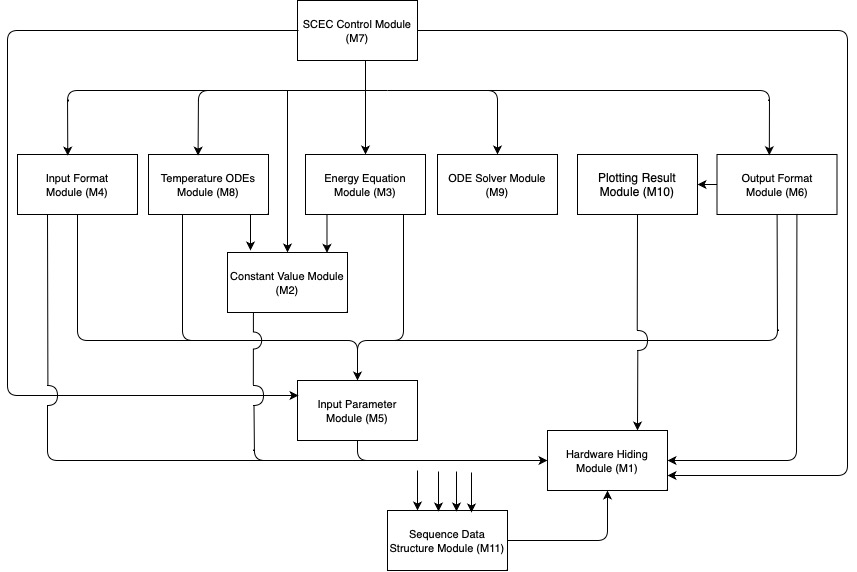
\includegraphics[width=0.7\textwidth]{HierchyModule.jpg}
\caption{Use Hierarchy Among Modules}
\label{FigUH}
\end{figure}

%\section*{References}
\newpage
\bibliographystyle {plainnat}
\bibliography {srs}

\newpage{}

\end{document}
